\documentclass[8pt,a4paper,compress]{beamer}

\usepackage{/home/siyer/lib/slides}

\title{Minimum Spanning Trees}
\date{}
\begin{document}
\begin{frame}
\vfill
\titlepage
\end{frame}

\begin{frame}
\frametitle{Outline}
\tableofcontents
\end{frame}

\section{What are Minimum Spanning Trees?}
\begin{frame}[fragile]
\pause

A spanning tree of a graph is a connected subgraph with no cycles that includes all the vertices

\pause
\bigskip

A minimum spanning tree (MST) of an edge-weighted undirected graph is a spanning tree whose weight (the sum of the weights of its edges) is no larger than the weight of any other spanning tree

\pause
\bigskip

An edge-weighted graph and its MST
\begin{minipage}{150pt}
\begin{lstlisting}[language={}]
$ more tinyEWG.txt 
8
16
4 5 0.35
4 7 0.37
5 7 0.28
0 7 0.16
1 5 0.32
0 4 0.38
2 3 0.17
1 7 0.19
0 2 0.26
1 2 0.36
1 3 0.29
2 7 0.34
6 2 0.40
3 6 0.52
6 0 0.58
6 4 0.93
\end{lstlisting}
\end{minipage}%
\begin{minipage}{150pt}
\begin{center}
\visible<4->{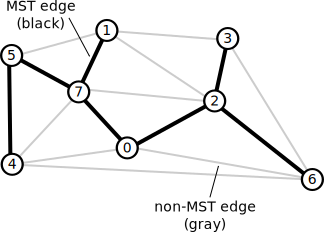
\includegraphics[scale=0.45]{{./figures/mst1}.pdf}}
\end{center}
\end{minipage}
\end{frame}

\begin{frame}[fragile]
\pause

If the graph is connected and the edge weights are unique, then MST exists and is unique

\pause
\bigskip

Goal: given a connected undirected graph $G$ with arbitrary (but distinct) edge weights, find the MST of $G$

\pause
\bigskip

Typical MST applications
\begin{center}
\begin{tabular}{ccc}
application & vertex & edge \\ \hline
circuit & component & wire \\
airline & airport & flight route \\
power distribution & power plant & transmission lines \\
image analysis & feature & proximity relationship
\end{tabular}
\end{center}
\end{frame}

\section{Edge-Weighted Graph API}
\begin{frame}
\pause

Weighted-edge data type (API)
\begin{center}
\begin{tabular}{cc}
method & description \\ \hline 
\lstinline$Edge(int v, int w, double weight)$ & create a weighted edge $v$-$w$ \\
\lstinline$double weight()$ & edge weight \\
\lstinline$int either()$ & either endpoint \\
\lstinline$int other(int v)$ & the endpoint that's not $v$
\end{tabular}  
\end{center}
\end{frame}

\begin{frame}[fragile]
\pause

Weighted-edge data type (implementation)
\begin{lstlisting}[language=Java]
package edu.princeton.cs.algs4;

public class Edge implements Comparable<Edge> {
    private final int v, w;
    private final double weight;

    public Edge(int v, int w, double weight) {
        if (v < 0 || w < 0) { throw new IndexOutOfBoundsException(); }
        if (Double.isNaN(weight)) { throw new IllegalArgumentException(); }
        this.v = v; this.w = w; this.weight = weight;
    }

    public double weight() { return weight; }

    public int either() { return v; }

    public int other(int vertex) {
        if      (vertex == v) { return w; }
        else if (vertex == w) { return v; }
        else { throw new IllegalArgumentException(); }
    }

    public int compareTo(Edge that) {
        if      (this.weight() < that.weight()) { return -1; }
        else if (this.weight() > that.weight()) { return +1; }
        else                                    { return  0; }
    }
}
\end{lstlisting}
\end{frame}

\begin{frame}[fragile]
\pause

Edge-weighted graph (API)

\begin{center}
\begin{tabular}{cc}
method & description \\ \hline
\lstinline$EdgeWeightedGraph(int V)$ & create an empty graph with $V$ vertices \\
\lstinline$EdgeWeightedGraph(In in)$ & create a graph from input stream \\
\lstinline$int V()$ & number of vertices  \\
\lstinline$int E()$ & number of edges \\
\lstinline$void addEdge(Edge e)$ & add weighted edge $e$ to this graph \\
\lstinline$Iterable<Edge> adj(int v)$ & edges incident to $v$ \\
\lstinline$Iterable<Edge> edges()$ & all edges in this graph
\end{tabular}  
\end{center}
\end{frame}

\begin{frame}[fragile]
\pause

Edge-weighted graph (implementation)
\begin{lstlisting}[language=Java]
package edu.princeton.cs.algs4;

public class EdgeWeightedGraph {
    private final int V;
    private int E;
    private LinkedBag<Edge>[] adj;
    
    public EdgeWeightedGraph(int V) {
        if (V < 0) { throw new IllegalArgumentException(); }
        this.V = V;
        this.E = 0;
        adj = (LinkedBag<Edge>[]) new LinkedBag[V];
        for (int v = 0; v < V; v++) {
            adj[v] = new LinkedBag<Edge>();
        }
    }

    public EdgeWeightedGraph(In in) {
        this(in.readInt());
        int E = in.readInt();
        if (E < 0) { throw new IllegalArgumentException(); }
        for (int i = 0; i < E; i++) {
            int v = in.readInt();
            int w = in.readInt();
            double weight = in.readDouble();
            Edge e = new Edge(v, w, weight);
            addEdge(e);
        }
    }
    
    public int V() { return V; }

    public int E() { return E; }
\end{lstlisting}
\end{frame}

\begin{frame}[fragile]
\pause

\begin{lstlisting}[language=Java]
    public void addEdge(Edge e) {
        int v = e.either();
        int w = e.other(v);
        validateVertex(v);
        validateVertex(w);
        adj[v].add(e);
        adj[w].add(e);
        E++;
    }

    public Iterable<Edge> adj(int v) {
        validateVertex(v);
        return adj[v];
    }

    public Iterable<Edge> edges() {
        LinkedBag<Edge> list = new LinkedBag<Edge>();
        for (int v = 0; v < V; v++) {
            int selfLoops = 0;
            for (Edge e : adj(v)) {
                if (e.other(v) > v) { list.add(e); }
                else if (e.other(v) == v) {
                    if (selfLoops % 2 == 0) { list.add(e); }
                    selfLoops++;
                }
            }
        }
        return list;
    }
}
\end{lstlisting}
\end{frame}

\section{Minimum Spanning Tree API}
\begin{frame}[fragile]
\pause

MST API
\begin{center}
\begin{tabular}{cc}
method & description \\ \hline
\lstinline$MST(EdgeWeightedGraph G)$ & constructor \\
\lstinline$Iterable<Edge> edges()$ & all of the MST edges \\
\lstinline$double weight()$ & weight of MST
\end{tabular}  
\end{center}

\pause

MST test client
\begin{lstlisting}[language=Java]
package edu.princeton.cs.algs4;

public class KruskalMST {
    public static void main(String[] args) {
        In in = new In(args[0]);
        EdgeWeightedGraph G = new EdgeWeightedGraph(in);
        MST mst = new MST(G);
        for (Edge e : mst.edges()) { 
            StdOut.println(e);
        }
        StdOut.println(mst.weight());
    }
}
\end{lstlisting}

\pause

\begin{lstlisting}[language={}]
$ java edu.princeton.cs.algs4.KruskalMST tinyEWG.txt
0-7 0.16
1-7 0.19
0-2 0.26
2-3 0.17
5-7 0.28
4-5 0.35
6-2 0.40
1.81
\end{lstlisting}
\end{frame}

\section{Greedy Algorithm}
\begin{frame}
\pause

\begin{minipage}{160pt}
A cut of a graph is a partition of its vertices into two nonempty disjoint sets

\pause
\bigskip

A crossing edge of a cut is an edge that connects a vertex in one set with a vertex in the other

\pause
\bigskip

Cut property: given any cut, a crossing edge of minimum weight is in the MST
\end{minipage}%
\begin{minipage}{140pt}
\begin{center}
\hfill \visible<2->{\includegraphics[scale=0.4]{{./figures/mst2}.pdf}}
\end{center}
\end{minipage}
\end{frame}

\begin{frame}[fragile]
\pause

\begin{minipage}{200pt}
Greedy MST algorithm
\begin{itemize}
\item Start with all edges colored gray

\item Find cut with no black edges and color its minimum-weight edge black

\item Repeat until $V - 1$ edges are colored black
\end{itemize}

\pause
\bigskip

The greedy algorithm computes the MST

\pause
\bigskip

Kruskal's algorithm that we consider next chooses cuts and minimum-weight edges efficiently
\end{minipage}%
\begin{minipage}{100pt}
\begin{center}
\visible<2->{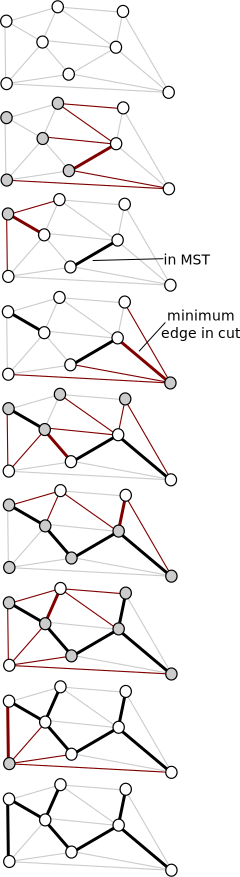
\includegraphics[scale=0.35]{./figures/mst3.pdf}}
\end{center}
\end{minipage}
\end{frame}

\section{Kruskal's Algorithm}
\begin{frame}[fragile]
\pause

Add edges to tree $T$ in ascending order of weight unless doing so would create a cycle

\pause
\bigskip

\begin{lstlisting}[language=Java]
package edu.princeton.cs.algs4;

public class KruskalMST {
    private double weight;  
    private LinkedQueue<Edge> mst;
    
    public KruskalMST(EdgeWeightedGraph G) {
        mst =  new LinkedQueue<Edge>();  
        MinPQ<Edge> pq = new MinPQ<Edge>();
        for (Edge e : G.edges()) { pq.insert(e); }
        WeightedQuickUnionUF uf = new WeightedQuickUnionUF(G.V());
        while (!pq.isEmpty() && mst.size() < G.V() - 1) {
            Edge e = pq.delMin();
            int v = e.either();
            int w = e.other(v);
            if (!uf.connected(v, w)) { 
                uf.union(v, w); 
                mst.enqueue(e); 
                weight += e.weight();
            }
        }
    }

    public Iterable<Edge> edges() { return mst; }

    public double weight() { return weight; }
}
\end{lstlisting}

\pause
\bigskip

Kruskal's algorithm computes MST in time proportional to
$E \log E$ in the worst case
\end{frame}

\begin{frame}[fragile]
\pause

Trace
\begin{center}
\visible<2->{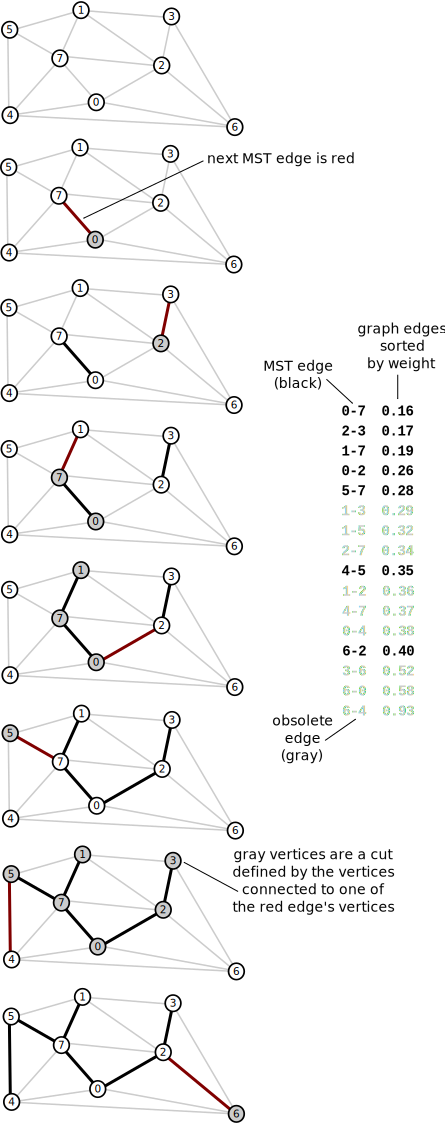
\includegraphics[scale=0.27]{./figures/mst4.pdf}}
\end{center}
\end{frame}
\end{document}
